%%%%%%%%%%%%%%%%%%%%%%%%%%%%%%%%%%%%%%%%%%%%%%%%%%%%%%%%%%%%%%%%%%%%%%%%
%%%  THIS TEX FILE IS TO GENERATE PDF FILE FOR 
%%% 
%%%  COPYRIGHT (C) JIMMY LIN, 2013, UT AUSTIN
%%%%%%%%%%%%%%%%%%%%%%%%%%%%%%%%%%%%%%%%%%%%%%%%%%%%%%%%%%%%%%%%%%%%%%%%
\documentclass[11pt,a4paper]{article}
%%%%%%%%%%%%%%%%%%%%%%%%%%%%%%%%%%%%%%%%%%%%%%%%%%%%%%%%%%%%%%%%%%%%%%%%
%%%  PACKAGES USED IN THIS TEX SOURCE FILE
%%%%%%%%%%%%%%%%%%%%%%%%%%%%%%%%%%%%%%%%%%%%%%%%%%%%%%%%%%%%%%%%%%%%%%%%
\usepackage{geometry,amsthm,amsmath,graphicx,amssymb,fancyheadings}
\usepackage[]{mcode}
\usepackage[colorlinks,
            linkcolor=blue,
            anchorcolor=red,
            citecolor=green
            ]{hyperref}
% for my mac
\IfFileExists{/Users/JimmyLin/.latex/UTA_CS/JS.sty}{ 
    \usepackage{/Users/JimmyLin/.latex/UTA_CS/JS}
    \usepackage{/Users/JimmyLin/.latex/UTA_CS/JSASGN}
}{} 
% for UT's linux machine
\IfFileExists{/u/jimmylin/workspace/Configs/latex/UTA_CS/JS.sty}{
    \usepackage{/u/jimmylin/.latex/UTA_CS/JS} 
    \usepackage{/u/jimmylin/.latex/UTA_CS/JSASGN}
}{} 
%%%%%%%%%%%%%%%%%%%%%%%%%%%%%%%%%%%%%%%%%%%%%%%%%%%%%%%%%%%%%%%%%%%%%%%%
%%% MACROS CONTAINING THE FILE INFORMATION
%%%%%%%%%%%%%%%%%%%%%%%%%%%%%%%%%%%%%%%%%%%%%%%%%%%%%%%%%%%%%%%%%%%%%%%%
\renewcommand{\COURSE}{EE381V Large Scale Optimization}
\renewcommand{\LECTURER}{Sujay Sanghavi}
\renewcommand{\SECTION}{17350}
\renewcommand{\TASK}{Problem Set 1}
\renewcommand{\RELEASEDATE}{September 12, 2014}
\renewcommand{\DUEDATE}{September 18, 2014}
\renewcommand{\TIMECONSUME}{10 hours}
%%%%%%%%%%%%%%%%%%%%%%%%%%%%%%%%%%%%%%%%%%%%%%%%%%%%%%%%%%%%%%%%%%%%%%%%
%%% DOCUMENTATION STARTS FROM HERE 
%%%%%%%%%%%%%%%%%%%%%%%%%%%%%%%%%%%%%%%%%%%%%%%%%%%%%%%%%%%%%%%%%%%%%%%%
\begin{document}
%%%%%%%%%%%%%%%%%%%%%%%%%%%%%%%%%%%%%%%%%%%%%%%%%%%%%%%%%%%%%%%%%%%%%%%%
%% TITLE PAGE
%%%%%%%%%%%%%%%%%%%%%%%%%%%%%%%%%%%%%%%%%%%%%%%%%%%%%%%%%%%%%%%%%%%%%%%%
\begin{titlepage}
    \maketitle
\end{titlepage}
%%%%%%%%%%%%%%%%%%%%%%%%%%%%%%%%%%%%%%%%%%%%%%%%%%%%%%%%%%%%%%%%%%%%%%%%
%% CONTENT PAGE: TABLEOFCONTENTS, LISTOFTABLES, LIST OF FIGURES
%%%%%%%%%%%%%%%%%%%%%%%%%%%%%%%%%%%%%%%%%%%%%%%%%%%%%%%%%%%%%%%%%%%%%%%%
\renewcommand{\contentsname}{Table of Contents}
\begin{center} 
    \tableofcontents 
    %\listoftables 
    \listoffigures
\end{center}
\newpage
%%%%%%%%%%%%%%%%%%%%%%%%%%%%%%%%%%%%%%%%%%%%%%%%%%%%%%%%%%%%%%%%%%%%%%%%
%%% GENERAL DOCUMENTATION BEGINS 
%%%%%%%%%%%%%%%%%%%%%%%%%%%%%%%%%%%%%%%%%%%%%%%%%%%%%%%%%%%%%%%%%%%%%%%%

\part{Matlab and Computational Assignment}
\section{Gradient Descent on three matrices}
Command to get executed: 
\begin{verbatim}
   >> gd_run_script()
\end{verbatim}
\subsection{$X1$, $b1$}
\begin{itemize}
    \item Range of $\gamma$ that leads to convergence: $(0,2)$
    \item Range of $\gamma$ that leads to divergence: $(2,+\infty)$
    \item Explanation: if $\gamma = 2$, the program indicates that 
        $$ \forall k,\ f(x^{k+1}) = f(x^{k})$$ 
        Since the above equation is constantly true (independent of the
        minima), we can conclude that gradient descent with $\gamma = 2$ goes 
        to the opposite side of that quadratic curve. Intuitively, the program 
        will diverge if we set larger ($\gamma>2$) and converge if we set smaller
        ($\gamma<2$).   
    \item Two illustrative examples: $\gamma = 0.5$ and $\gamma = 3.0$
        \begin{figure}[h]
            \centering
            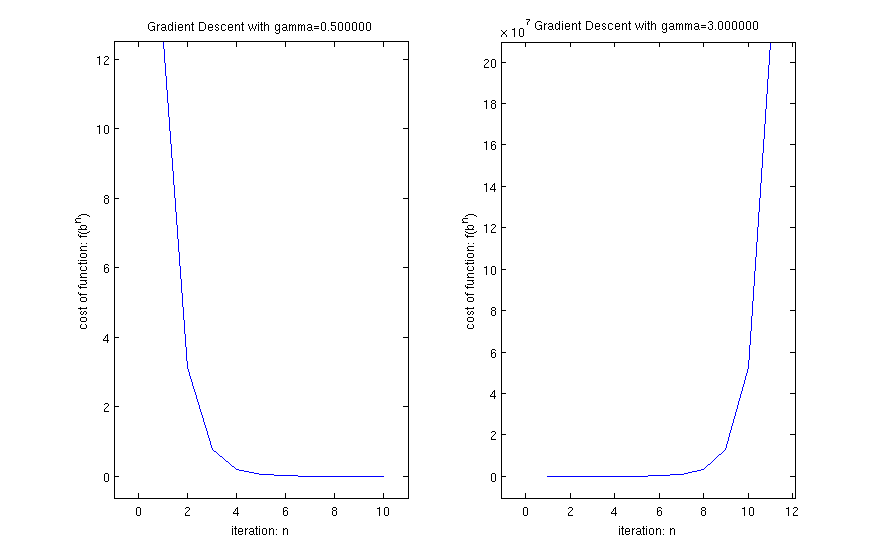
\includegraphics[width=6in,height=3in]{../ps1_matlab/1.png}
            \caption{Illustration for gradient descent on $X1$, staring with
                $b1$ by $\gamma = 0.5$ and $3.0$}
        \end{figure}
\end{itemize}

\newpage
\subsection{$X2$, $b2$}
\begin{itemize}
    \item Range of $\gamma$ that leads to convergence: $(0,2)$
    \item Range of $\gamma$ that leads to divergence: $(2,+\infty)$
    \item Explanation: if $\gamma = 2$, the program indicates that 
        $$ \forall k,\ f(x^{k+1}) = f(x^{k})$$ 
        Since the above equation is constantly true (independent of the
        minima), we can conclude that gradient descent with $\gamma = 2$ goes 
        to the opposite side of that quadratic curve. Intuitively, the program 
        will diverge if we set larger ($\gamma>2$) and converge if we set smaller
        ($\gamma<2$).
    \item Two illustrative
        examples: $\gamma = 1.5$ and $\gamma = 3.0$
        \begin{figure}[h]
            \centering
            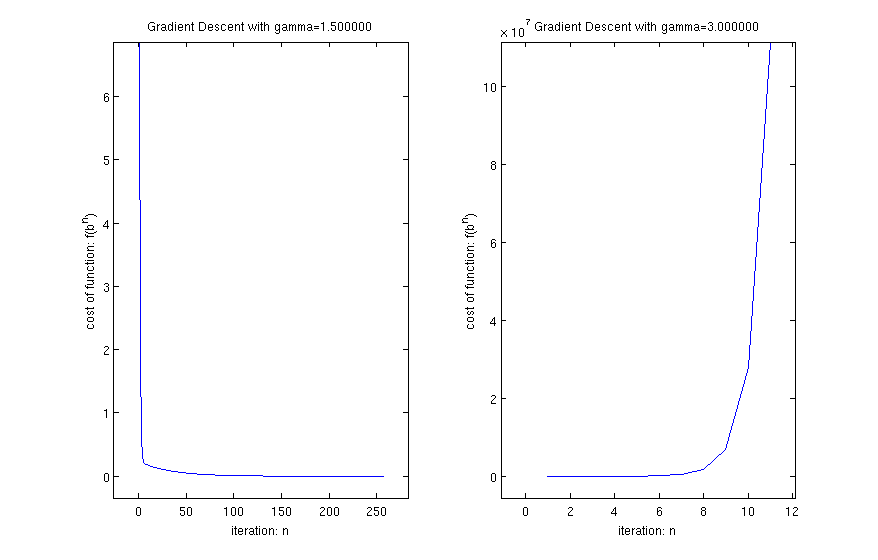
\includegraphics[width=6in,height=3in]{../ps1_matlab/2.png}
            \caption{Illustration for gradient descent on $X2$, starting with
                $b2$ by $\gamma = 1.5$ and $3.0$}
        \end{figure}
\end{itemize}

\newpage
\subsection{$X3$, $b3$}
\begin{itemize}
    \item Range of $\gamma$ that leads to convergence: $(0,0.02)$
    \item Range of $\gamma$ that leads to divergence: $(0.02,+\infty)$
    \item Explanation: if $\gamma = 0.02$, the program indicates that 
        $$ \forall k,\ f(x^{k+1}) = f(x^{k})$$ 
        Since the above equation is constantly true (independent of the
        minima), we can conclude that gradient descent with $\gamma = 0.02$ goes 
        to the opposite side of that quadratic curve. Intuitively, the program 
        will diverge if we set larger ($\gamma>0.02$) and converge if we set smaller
        ($\gamma<0.02$).
    \item Two illustrative examples: $\gamma = 0.005$ and $\gamma = 0.05$
        \begin{figure}[h]
            \centering
            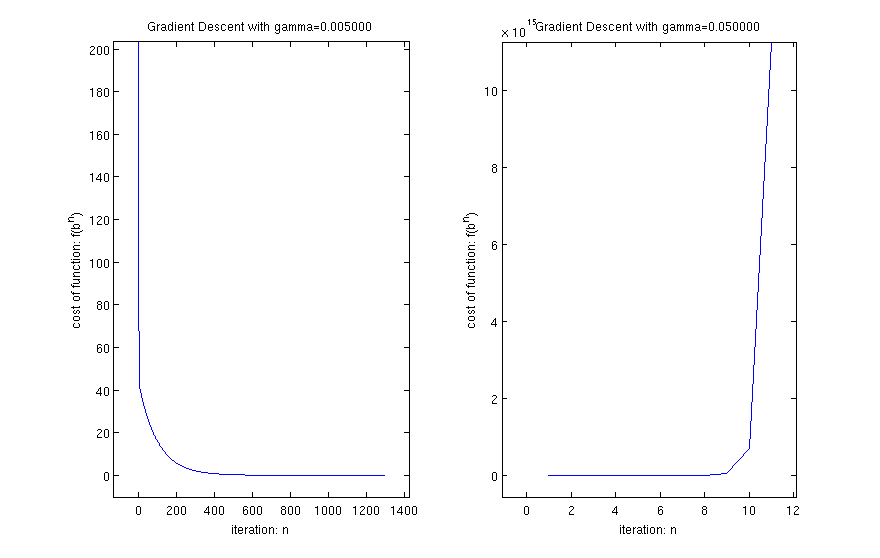
\includegraphics[width=6in,height=3in]{../ps1_matlab/3.png}
            \caption{Illustration for gradient descent on $X3$ staring with
                $b3$ by $\gamma = 0.005$ and $0.05$}
        \end{figure}
\end{itemize}

\newpage
\section{$\gamma = 1$ for the second matrix}
Command to get executed: 
\begin{verbatim}
   >> [b2_opt, iters, all_costs] = gd (X2, b2, 1);
\end{verbatim}
{\bf Plotting}: figure for $\gamma = 1$
\begin{figure}[h]
            \centering
            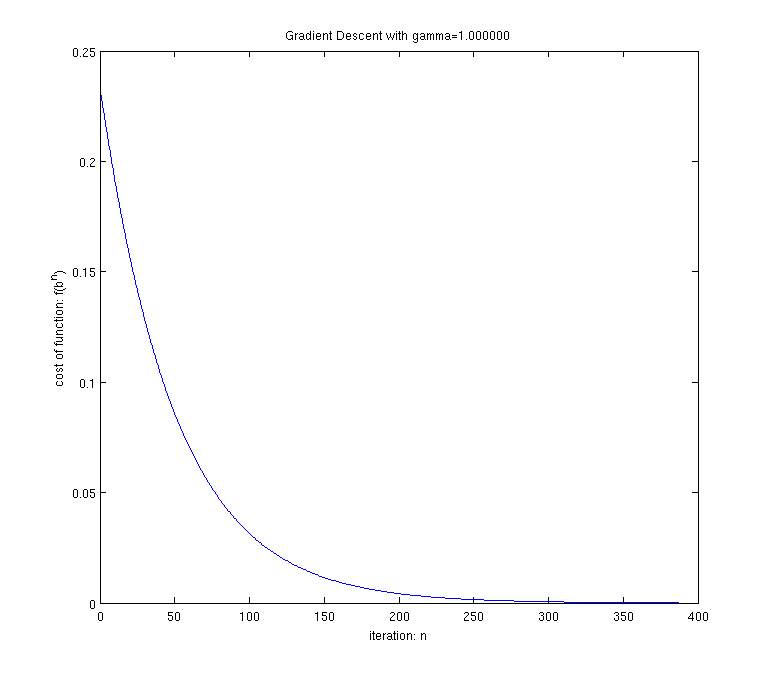
\includegraphics[width=4in,height=3in]{../ps1_matlab/2_gamma1.png}
            \caption{Plotting figure for gradient descent with $\gamma = 1$ on
            the second matrix}
\end{figure}

\noindent
{\bf Explanation}: 
Through the smooth plotted curve, we guess that the gradient
descent method got linear convergence when $\gamma=1$ on $X_2$. Hence, we trace
convergence rate conv\_rate $ = f(x^{k}) / f(x^{k-1})$ as follows:
\begin{verbatim}
Iter: 2, Cost: 2.254428e-01, Conv_Rate: 0.980100
Iter: 3, Cost: 2.209565e-01, Conv_Rate: 0.980100
Iter: 4, Cost: 2.165594e-01, Conv_Rate: 0.980100
Iter: 5, Cost: 2.122499e-01, Conv_Rate: 0.980100
Iter: 6, Cost: 2.080261e-01, Conv_Rate: 0.980100
Iter: 7, Cost: 2.038864e-01, Conv_Rate: 0.980100
...
...
Iter: 381, Cost: 1.107934e-04, Conv_Rate: 0.980100
Iter: 382, Cost: 1.085886e-04, Conv_Rate: 0.980100
Iter: 383, Cost: 1.064277e-04, Conv_Rate: 0.980100
Iter: 384, Cost: 1.043098e-04, Conv_Rate: 0.980100
Iter: 385, Cost: 1.022340e-04, Conv_Rate: 0.980100
Iter: 386, Cost: 1.001996e-04, Conv_Rate: 0.980100
Iter: 387, Cost: 9.820558e-05, Conv_Rate: 0.980100
Converged to zeros!
\end{verbatim}
In terms of above dumps and the fact that $f(x^{*}) = 0$, we can conclude that when $\gamma = 1$        
$$
f(x^{k+1}) - f(x^{*}) = 0.9801 \cdot \big( f(x^{k}) - f(x^{*}) \big)
$$
which supports our previous guess that
$$ 
\text{Gradient Descent with }
\gamma = 1
\text{ on second matrix leads to {\bf linear convergence}. }
$$

\newpage
%%%%%%%%%%%%%%%%%%%%%%%%%%%%%%%%%%%%%%%%%%%%%%%%%%%%%%%%%%%%
%%% Written Problems
%%%%%%%%%%%%%%%%%%%%%%%%%%%%%%%%%%%%%%%%%%%%%%%%%%%%%%%%%%%%
\newpage
\part{Written Problems}
\setcounter{section}{0}
\renewcommand{\thesubsection}{(\alph{subsection})}
\section{Othorognal Subspace}
\newcommand{\Ut}{U^{\perp}}
\newcommand{\ut}{u^{\perp}}
\newcommand{\Wt}{W^{\perp}}
\newcommand{\Xt}{X^{\perp}}
\newcommand{\zerovec}{\mathbf{0}} 
\newcommand{\uvec}{\mathbf{u}}
\newcommand{\vvec}{\mathbf{v}}
\newcommand{\xvec}{\mathbf{x}}
\subsection{Show that if $U$ is a subspace, then so is $\Ut$}
\begin{proof}
    Since $U$ is a subspace, then we have $U$ satisfying all three properties
    shown below:
    \begin{itemize}
       \item $\zerovec \in U$ 
       \item $\forall \uvec_1, \uvec_2 \in U, \uvec_1 + \uvec_2 \in U$
       \item $\forall \uvec \in U, \alpha \in \mathbb{R}, \alpha \uvec \in U$
    \end{itemize}
    Now we show that $\Ut$ is also a subspace by indicating $\Ut$
    satisfies all three properties as above $U$ do.
    \begin{itemize}
        \item Since $\forall \uvec \in U, \langle \zerovec, \uvec \rangle = 0$
            and $\zerovec \in V$ ($\zerovec \in U \subseteq V$), then it
            turned out that $\zerovec \in \Ut$.
        \item Let $\uvec$ be arbitrary vector s.t. $\uvec \in U$, and
            $\xvec_1$, $\xvec_2$ to be distinct vector s.t. $\xvec_1 \in \Ut$
            and $\xvec_2 \in \Ut$. By definition of $\Ut$, we have 
            $\langle \xvec_1, \uvec \rangle = 0$ and 
            $\langle \xvec_2, \uvec \rangle = 0$. 
            Then it is obvious that 
            $\langle \xvec_1 + \xvec_2, \uvec \rangle = 0$. 
            That is $\xvec_1 +\xvec_2 \in \Ut$.
            Therefore, $\forall \xvec_1, \xvec_2 \in \Ut, \xvec_1+\xvec_2 \in \Ut$ was proved.
        \item Let $\xvec$ be arbitrary vector s.t. $\xvec \in \Ut$, 
            $\uvec$ be arbitrary vector s.t. $\uvec \in U$ and
            arbitrary $\alpha \in \mathbb{R}$. By definition of $\Ut$, we have 
            $\langle \xvec_1, \uvec \rangle = 0$. 
            Since inner product is linear operator, it is obvious that
            $\langle \alpha \xvec_1, \uvec \rangle = 0$. 
            That is $\alpha \xvec_1 \in \Ut$.
            Therefore, $\forall \xvec \in \Ut, \alpha \in \mathbb{R}, \alpha
            \xvec \in \Ut$ was proved.
    \end{itemize}
    Since $\Ut$ contains $\zerovec$, and is closed under addition and scalar
    multiplication, it turned out that $\Ut$ is a subspace. 
    Therefore, the statement that if $U$ is a subspace, then so is $\Ut$ was
    proved.
\end{proof}
\subsection{Show that $(\Ut)^{\perp} = U$}
\begin{proof}[Proof by contradiction.]
    Assume that $(\Ut)^{\perp} \not= U$ and then show the contradiction. 
    By definition of $\Ut$, we have
    $ \Ut = 
    \{\forall \vvec, \langle \vvec, \uvec \rangle = 0, \forall \uvec \in U\}$
    and 
    $ (\Ut)^{\perp} = 
    \{\forall \xvec, \langle \xvec, \vvec \rangle = 0, \forall \vvec \in \Ut\}$.
    Since $(\Ut)^{\perp} \not= U$, then we can say that 
    $ \exists \xvec \not \in U, \langle \xvec, \vvec \rangle = 0, \forall
     \vvec \in \Ut $. 
     That is to say, 
    $ \exists \xvec \in V\ but\ \not \in U, \langle \xvec, \vvec \rangle = 0, \forall
     \vvec \ s.t. \langle \vvec, \uvec \rangle = 0, \forall \uvec \in U$. 
     However, such $\xvec$ does not exist. Hence, we reject
     initial assumption and conclude that $(\Ut)^{\perp} = U$.
\end{proof}

\subsection{Show that if $U, W \subseteq V$ are subspaces of V, then $U
    \subset W \Leftrightarrow \Ut \supseteq \Wt$}

\subsection{Show that $\Xt$ makes sense, $\Xt$ is a subspace and
    $(\Xt)^{\perp} \supseteq X$}

\subsection{Show that any $v \in V$ can be written uniquely as $v = u + \ut$} 

\newpage
\section{Boyd and Vandenberghe, Ex. 2.10}
\newcommand{\Snp}{\ensuremath{\mathbb{S}_{+}^{n}}}
\subsection{Show that if $A \in \Snp$ then the set C is
    convex}

\subsection{Show that $C_1$ is convex if there exists $\lambda \in
    \mathbb{R}$ such that $(A + \lambda gg^T) \in \Snp$}

\newpage
\section{Boyd and Vandenberghe, Ex. 2.21}

\newpage
\setcounter{section}{6}
\section{Form a Half-Space}

\newpage
\setcounter{section}{7}
\section{Exists $C$ such that $CA = B$}

\newpage
\appendix
\section{Codes Printout}

\subsection{Gradient Descent Routine}
\lstinputlisting{../ps1_matlab/gd.m}
\newpage

\subsection{Running Script}
\lstinputlisting{../ps1_matlab/gd_run_script.m}

%%%%%%%%%%%%%%%%%%%%%%%%%%%%%%%%%%%%%%%%%%%%%%%%%%%%%%%%%%%%%%%%%%%%%%%%
%%% General Documentation ends
%%%%%%%%%%%%%%%%%%%%%%%%%%%%%%%%%%%%%%%%%%%%%%%%%%%%%%%%%%%%%%%%%%%%%%%%
\end{document}
